%% sdb_final.tex
%% 2011/12/6
%% by William J. Woodall IV

\documentclass[journal]{IEEEtran}

%% For Citations
\usepackage{cite}

%% For graphics
\usepackage[pdftex]{graphicx}
\graphicspath{{images/}}
\DeclareGraphicsExtensions{.pdf,.jpeg,.png}

%% For URL's
\usepackage{url}

%% For Algorithms
\usepackage{algorithm}
\usepackage{algorithmic}

%% Set paper title
\newcommand{\ThisPaperTitle}
{Representing 3D Environments for Teleoperation of Robots using Octrees}

% correct bad hyphenation
\hyphenation{op-tical net-works semi-conduc-tor}

\begin{document}
  
  \title{\ThisPaperTitle{}}
  
  \author{William~J.~Woodall~IV}
  
  % Paper Header
  \markboth{COMP 7970 Trends in Spatial Databases}%
  {Woodall:\ThisPaperTitle{}}
  
  % Make room for the title
  \maketitle
  
  % Abstract
  \begin{abstract}
    This paper applies the octree data structure to the storage and
    transmission of three dimensional data to be used in the teleoperation of
    robotic vehicles. Three dimensional data from sensors like the Microsoft
    Kinect is paired with positional information from a robotic platform to
    reconstruct the environment and store it in an octree data structure. The
    environment is represented with an occupancy metric that is determined
    probabilistically by storing the probability of occupation for each leaf
    of the octree and then creating a maximum likelihood version of the
    resulting tree. For teleoperation of a robotic vehicle the octree
    representation of the environment needs to be synchronized across a
    potentially unreliable network. To do this the octrees need to be
    differenced, transmitted, and then united. This paper describes the
    experimental setup and results of the described teleoperation system.
  \end{abstract}
  
  % Keywords
  \begin{IEEEkeywords}
    Mapping, Teleoperation, Octree, Kinect, Robotics
  \end{IEEEkeywords}
  
  % Don't know if I need this...
  \IEEEpeerreviewmaketitle
  
  \section{Introduction}
  \IEEEPARstart{M}{apping} three dimensional environments has become a hot 
  research topic in the past few years, and some amount of that trend can be 
  attributed to the Microsoft Kinect.  Since its release in November of 
  2010\cite{GIZMODO}, the Kinect has enabled researchers and enthusiasts all 
  over the world by giving them access to high quality three dimensional data 
  in an available and affordable sensor package.  This paper takes advantage 
  of the innovation of the Kinect to apply this technology to the 
  teleoperation of mobile robot vehicles.  To facilitate this activity, 
  octrees are used to represent the environment and the reasons why this 
  design decision was made are covered in this paper.
  
  \subsection{Context}
  With the increasing availability of three dimensional spatial data from 
  sensors like the Primesense based RGB-Depth cameras \cite{PRIMESENSE} and 
  registering sweeping laser range finders with cameras \cite{5457431}, being 
  able to store, transmit and manipulate this data in an efficient manner has 
  become important.  There are a number of applications for this type of 3D 
  information, for example: 3D or 6D SLAM \cite{biswasdepth}, 3D 
  teleoperation \cite{5457431}, and robotic path planning \cite{3DCOLLISION}.
  This paper focuses on using the data for assisting teleoperation of 
  robot vehicles by providing a 3D representation of the environment.
  
  Outdoor and Indoor environments can be difficult to capture in full three 
  dimensional space.  One of the issues with mapping three dimensional 
  space is that the computing resources (like processing time, memory usage, 
  and network bandwidth) can be prohibitive to storing, transmitting, and 
  processing the map.  Octrees have a long history of being used in 3D 
  applications\cite{CITEME}, ranging from occupancy grids\cite{CITEME}, 
  surface reconstruction\cite{CITEME}, and computer graphics\cite{CITEME}.  
  Recent work has shown that arbitrary 3D maps can be stored efficiently using 
  octrees for use in robotics applications\cite{octomap}.  The research by A. 
  Hornung, et. al. resulted in an open source library called octomap 
  \cite{octomap}.  The primary use of the octomap library so far has been in 
  occupancy based motion planning for robots and robotic manipulators 
  \cite{3DCOLLISION}. This paper applies this octree based spatial database 
  methods described in the octomap paper to 3D teleoperation of robotic 
  vehicles.
  
  \subsection{System Overview}
  The teleoperation of robotic vehicles implies a client-server architecture 
  where one machine has the telemetry and another machine has the operator 
  which generates commands for the machine with the telemetry.  In the 
  simplest case a robot, or server, has proprioceptive and exteroception 
  sensors with which to locate itself and observe the environment, and 
  communicates this telemetry to an operator's computer, or client, which 
  visualize the telemetry and transmits user commands back to the server.  In 
  the system described in this paper a pair of robotic platforms based on the 
  Segway RMP base and the iRobot ATRV are used to collect, process, and 
  transmit the telemetry.  The telemetry is received by the client computer, 
  usually a laptop or workstation, and is displayed.
  
  \begin{figure}[here]
    \centering
    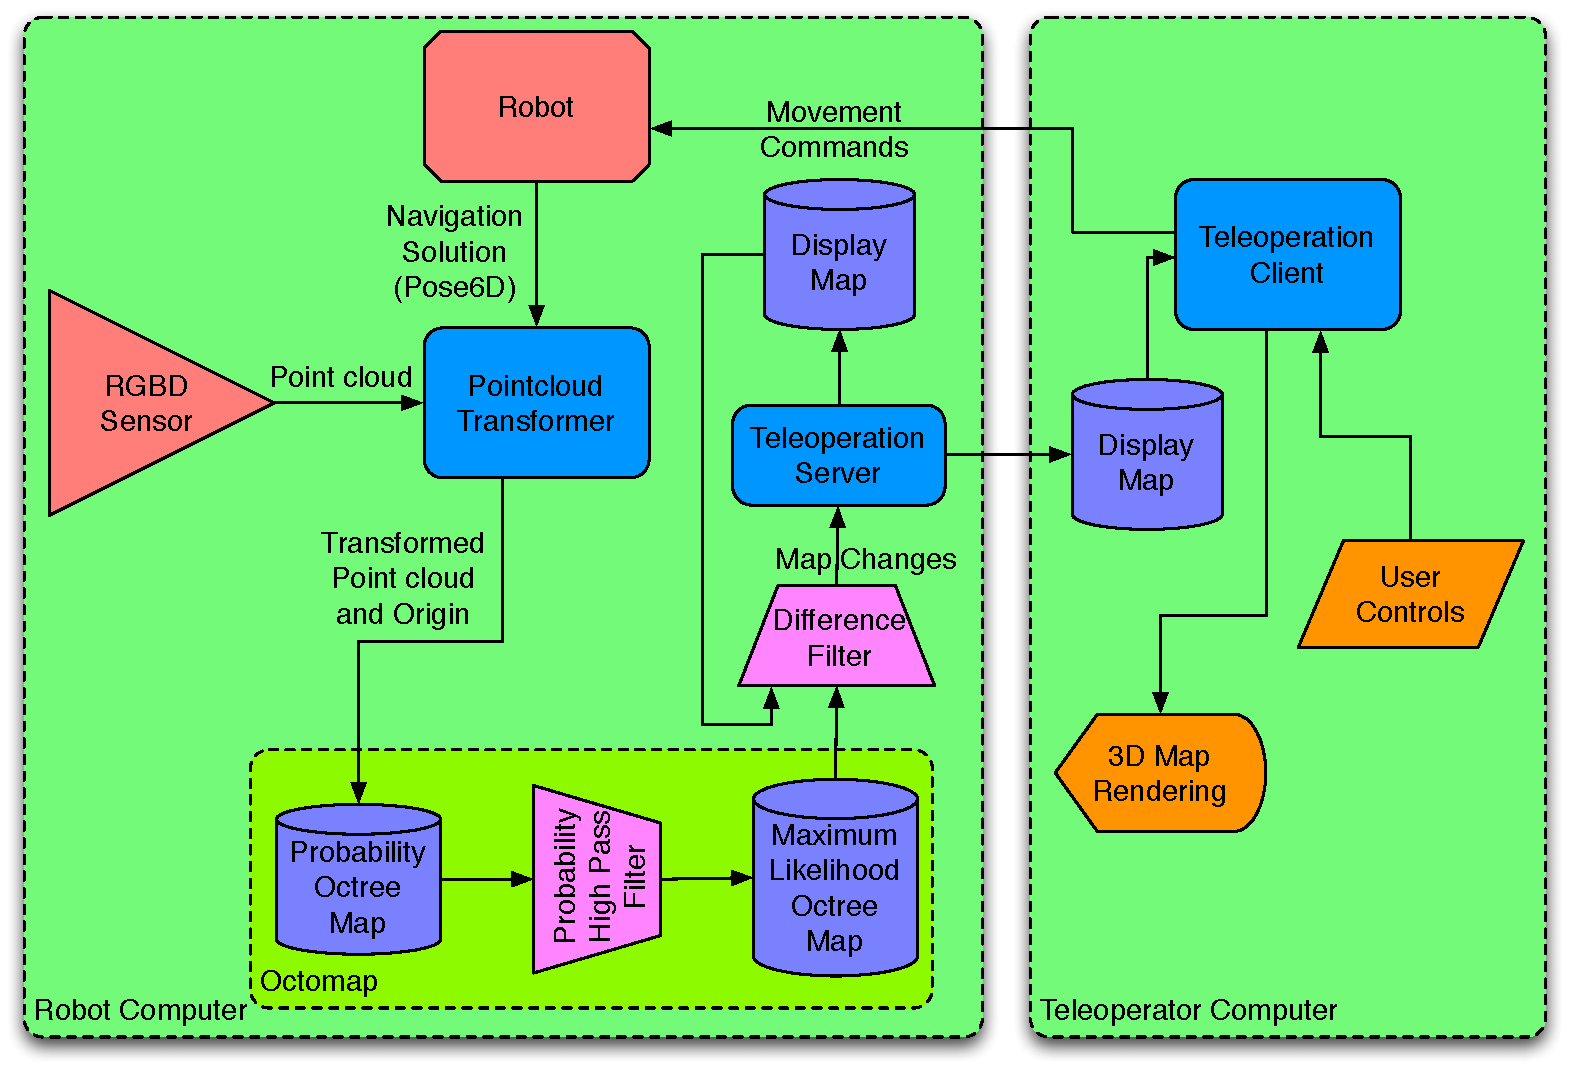
\includegraphics[width=3.5in,keepaspectratio]{system_diagram.pdf}
    \caption{System Design}
    \label{fig:system_diagram}
  \end{figure}
  
  Figure~\ref{fig:system_diagram} describes the overall system design.  The 
  three dimensional point clouds collected from a sensor, like the Microsoft 
  Kinect, are combined with a navigation solution from the robotic base to 
  transform the data points into a common map frame.  At this point the point 
  clouds are inserted into the map using octomap's probabilistic insertion 
  method.  A maximum likelihood version of the map is generated using octomap 
  and is stored as what this paper will refer to as the server map.  At this 
  point the map is ready to be used in teleoperation, so the server map is 
  subtracted from the map that the client current has, referred to as the 
  client map.  The differences, or part of the differences, are sent to the 
  client and united with the current client map.  If all of the differences 
  are sent, then the client map and the server map should then be 
  synchronized, otherwise successive iterations of this process should finally 
  result in an up-to-date client map.
  
  The rest of the paper will cover previous work, detail the three dimensional 
  mapping process, describe the teleoperation related activities in more 
  detail, and then describe some possible future work.
  
  \section{Previous Work}
  Each of the areas of this paper have some extensive previous work and the 
  major contribution is the combination of the technologies applied to 
  teleoperation of robotic vehicles.  This section will describe the previous 
  work for each of the relevant parts of the system.
  
  \subsection{Three Dimensional Mapping}
  \label{sec:previouswork_3dmapping}
  Recent work has been done to create three dimensional maps of the
  environment using octree's and a probabilistic insertion method that is well
  suited for robotic activities where there is noise in the data and
  uncertainty in the position of the robot. A. Hornung, et. al. described and
  implemented this system and it resulted in an open-source library called
  octomap.\cite{octomap} This paper uses octomap as the octree mapping system
  and exactly how that works is described in section \ref{sec:3dmapping}.
  There are two main elements of the octomap research that are useful in a
  three dimensional teleoperation system.
  
  First, the probabilistic method for adding new three dimensional information
  to the map is ideal for a system that needs to be updated continuously.
  Uncertainty from the navigation solution will result in point clouds that 
  are transformed slightly incorrect, and this causes inconsistencies and 
  skews in the resulting map. The probabilistic manner in which the scans are 
  inserted into the octree help to alleviate this inconsistency by allowing 
  for some error in the point clouds in relation to map. This is further 
  alleviated by the nature of the octree data structure, because inserting the 
  point clouds into the octree essentially results in a downsampling of the 
  original data.
  
  Second, the ability to limit the depth of a 3D query in order to control the 
  fidelity of the 3D representation of the environment allows for an 
  adjustable quality level to match the available resources like network 
  bandwidth and network latency.  This is important because most teleoperation 
  systems work over a wireless and unreliable communication layer, which often 
  suffers from low data rates and large latencies.  An analogy can be drawn to 
  how on-line video streaming services will adjust the compression of a video 
  to accommodate the connection being used, but in these systems the main 
  concern is bandwidth not latency.
  
  \subsection{Three Dimensional Teleoperation}
  Information about previous 3D work (CMU and maybe Florida)
  
  \section{Three Dimensional Mapping}
  \label{sec:3dmapping}
  This section describes the process of combining the three dimensional data
  from the sensor and six dimensional poses from the robot base into three
  dimensional maps of the environment. As previously mentioned in Section
  \ref{sec:previouswork_3dmapping} A. Hornung, et. al. have already shown that
  octrees combined with a probabilistic insertion method can provide a good
  solution when creating three dimensional maps in this manner. A majority of
  this section is just explaining their work and how it is used in the
  teleoperation system described in this paper.\cite{octomap} The obvious
  first steps of this process is obtaining the three dimensional data and the
  six dimensional pose of the robotic base from which the map is constructed,
  but these are described briefly in Section \ref{sec:experimental_setup}.
  
  \subsection{Transforming the Point Clouds}
  Each time new data from the three dimensional sensor is received by the
  robot computer the data needs to be rotated into a common map frame. Figure
  \ref{fig:transforms} shows a typical transformation tree for the robotic
  setup. The transformation between the map coordinate frame and the odom
  coordinate frame represents the accumulated error from the odometry of the
  robot that has been corrected by the localization algorithm. The
  transformation between the odom frame and the base link frame represents the
  accumulated absolute transformation given by the robot's odometry. The
  transforms between the base link frame and both the laser link frame and the
  openni camera frame are static geometric relation ships and represent the
  position of the sensors on the robot chassis. When new point clouds are
  receive they are in the openni camera coordinate frame and need to be
  converted into the map coordinate frame as that is the corrected global
  frame in this situation.
  
  \begin{figure}[here]
    \centering
    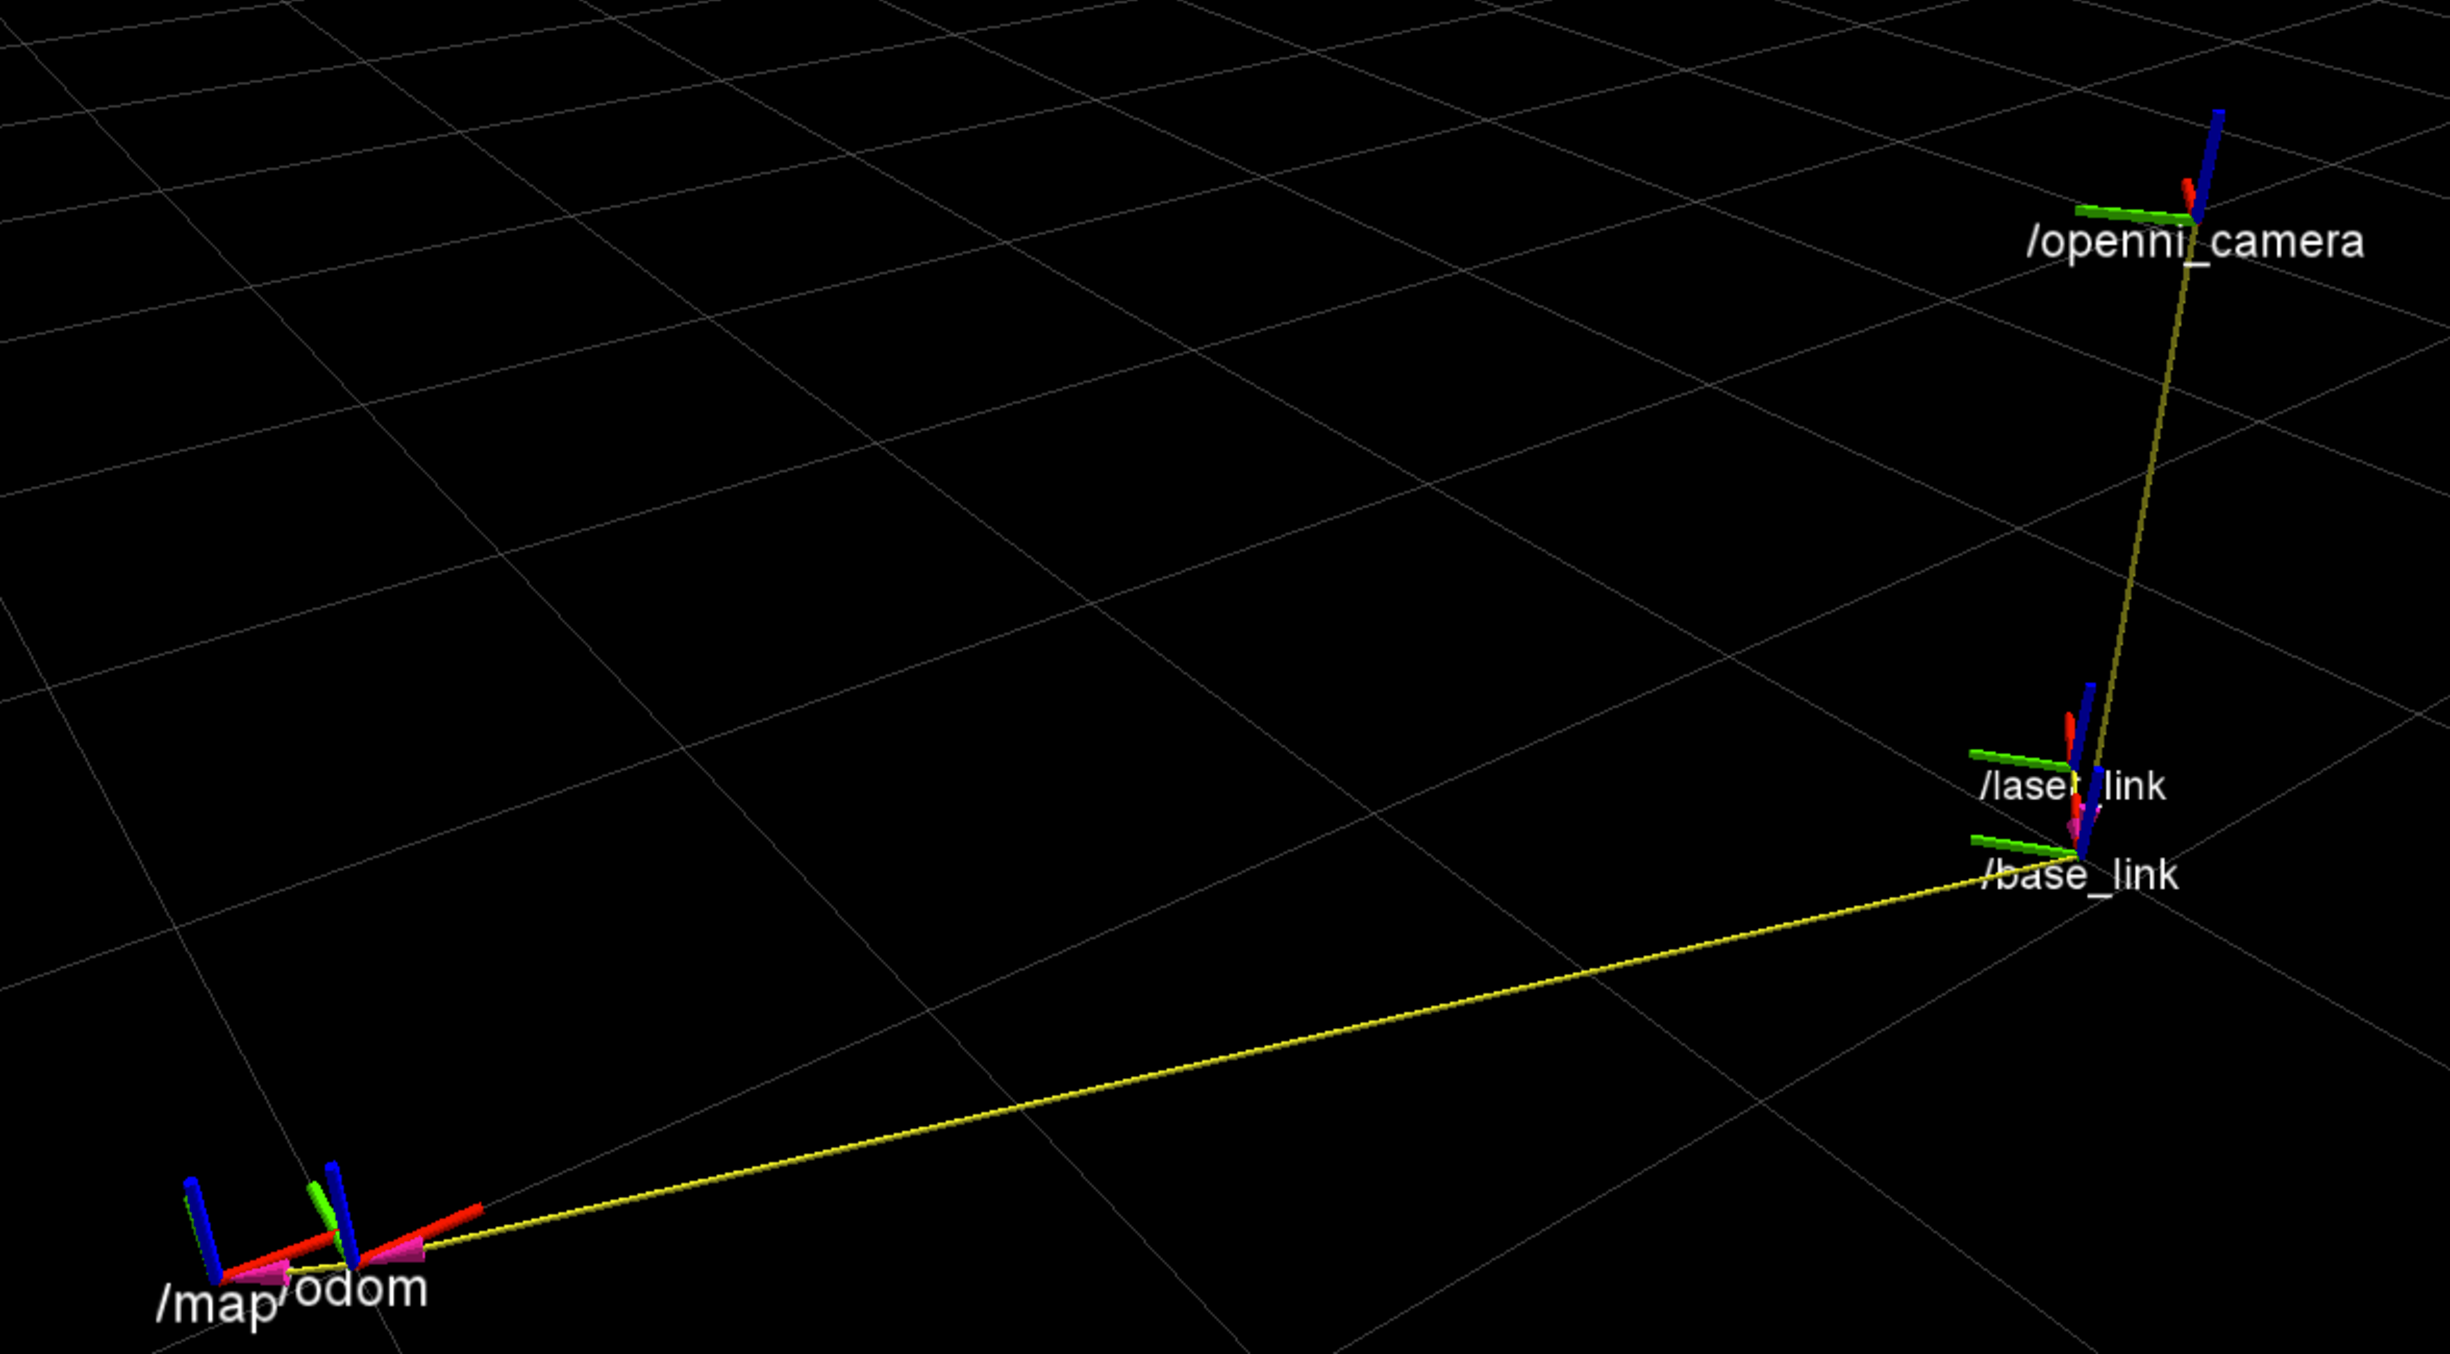
\includegraphics[width=3.5in,keepaspectratio]{transform.pdf}
    \caption{Typical Coordinate Transform Tree}
    \label{fig:transforms}
  \end{figure}
  
  \subsection{Inserting New Data}
  Once the point cloud data has been transformed into the global map
  coordinate frame the data needs to be added to the map. This is done by the
  octomap library, but I will describe the process here. The underlying data
  structure for this map is an octree where each leaf has a probability of
  occupation. This in effect is a three dimensional occupancy grid with octree
  storage where each leaf of the tree is a voxel in the grid. The transformed
  data and the origin of the sensor in the global map coordinate frame are
  required for the insertion. The insertion method starts by iteratively ray
  tracing from the origin of the sensor to each data point in the point cloud.
  For each voxel that the ray trace passes through the probability of
  occupation of for that voxel is decreased by a given amount. For the voxel
  that the ray trace ends in the probability of that voxel being occupied is
  increased by a given amount. In this way it takes several points falling
  into a voxel to have voxel considered to be occupied and allows for fringe
  voxels caused by noise to be cleared by additional new data. 
  
  \begin{figure}[here]
    \centering
    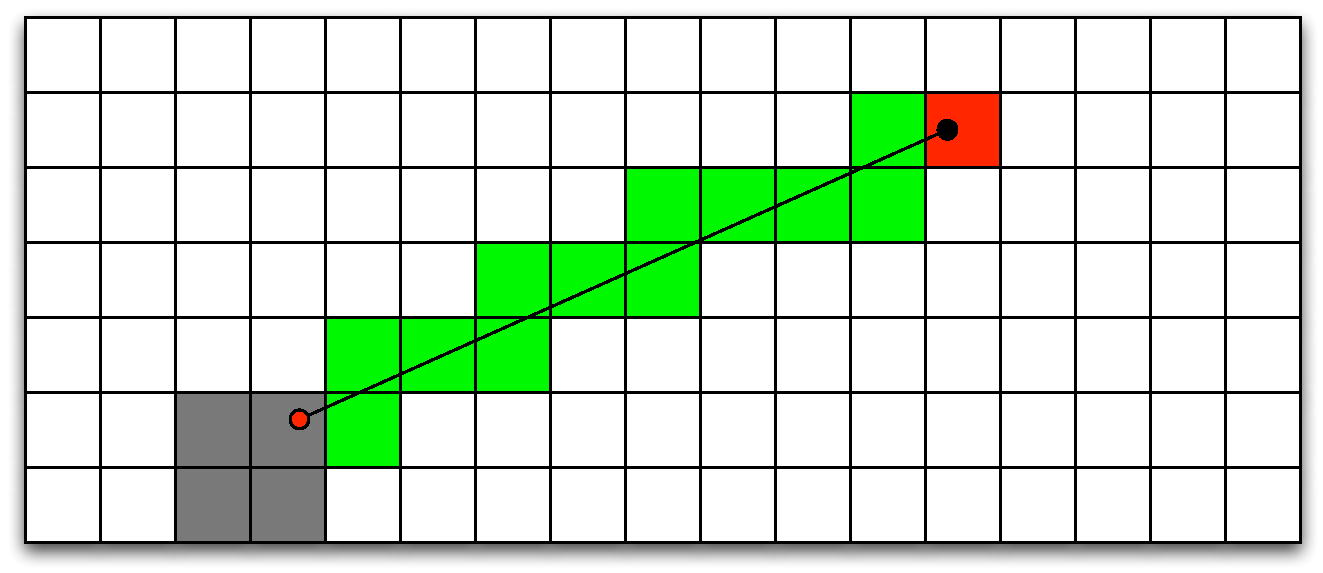
\includegraphics[width=3.5in,keepaspectratio]{raytrace.pdf}
    \caption{Two Dimensional Example of Voxel Raytracing}
    \label{fig:voxel_raytrace}
  \end{figure}
  
  Figure \ref{fig:voxel_raytrace} shows this process in a two dimensional
  example where the grey voxels are the robot, the red dot is the sensor
  origin, the black dot is the point from the point cloud, the green voxels
  are having their occupancy decreased, and the red voxel is having its
  occupancy increased. This method of voxel ray tracing is originally proposed
  by Amanatides, J. and Woo, A., and is referenced in the octomap
  paper.\cite{amanatides1987fast}
  
  \subsection{Error During Mapping}
  The results of the three dimensional mapping are dependent on several
  factors. The resulting map is sensitive to the vehicle position uncertainty
  and the sensor error. Figure \ref{fig:slamvsoctree} shows the resulting
  octree map with the map from the Simultaneous Localization and Mapping
  (SLAM) algorithm, which is good enough in this instance to be considered
  truth. The octree map generally lines up with the SLAM map but has a lot of
  areas where the result is less than desirable.
  
  \begin{figure}[here]
    \centering
    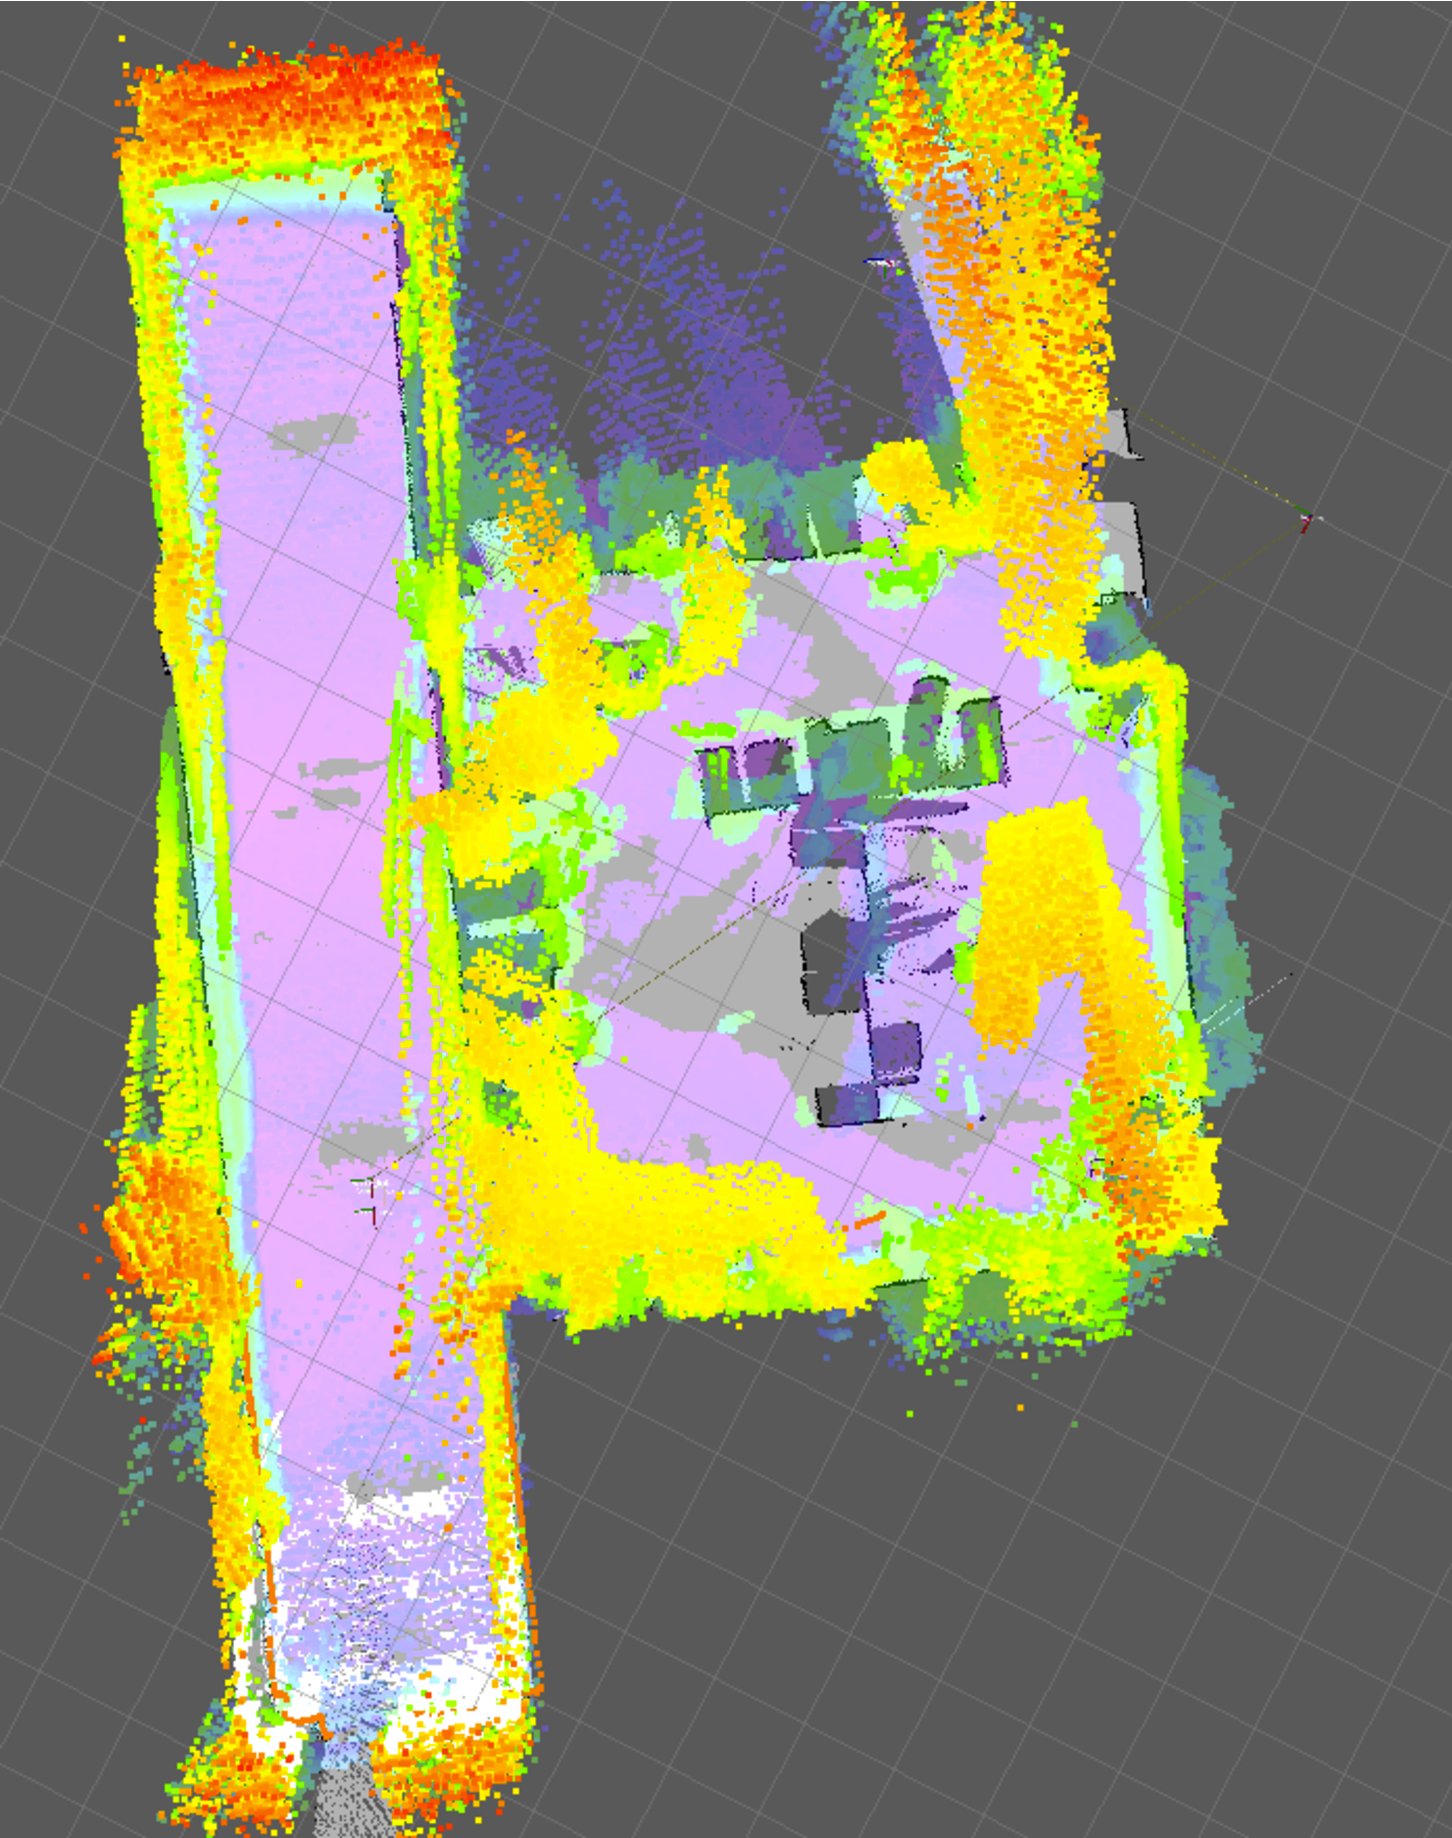
\includegraphics[width=3.5in,keepaspectratio]{slamvsoctree.pdf}
    \caption{Example of Three Dimensional Mapping with Test Data}
    \label{fig:slamvsoctree}
  \end{figure}
  
  \subsubsection{Vehicle Position Uncertainty}
  The main source of error in the map for real life test data in this paper is
  the uncertainty of the vehicle position. In Figure \ref{fig:slamvsoctree}
  the main areas that can be attributed to position error are where the octree
  map goes past the SLAM map and appears to have thick walls. This is because
  the robot was driving towards the wall and the position error changed as the
  robot moved towards the wall. This causes a linear smear effect, but this
  effect is not present on the interior because of the clearing behavior of
  the octree map.
  
  \subsubsection{Sensor Error}
  The secondary source of error in the real data is the noise on the sensor
  data. No sensor is perfect, but they do very considerably. The laser range
  finder used for the SLAM algorithm has a much tighter variance on the range
  estimates every at great distances. The Kinect, however, has considerably
  more noise, about 2cm of variance at 1.5 to 3 meters, but up to 4cm at
  ranges near the limit at around 6 meters.\cite{khoshelham2011accuracy} The
  error in the Kinect's data manifests in Figure \ref{fig:slamvsoctree} as
  high spatial frequency noise in the map and also contributes to the smearing
  that was mentioned in the previous section on Vehicle Position Uncertainty.
  
  \section{Teleoperation}
  While the three dimensional map is being continuously generated the client
  needs to be updated regularly so that the operator has useful information
  from which to command the robotic vehicle. This is where the application of
  the three dimensional mapping to teleoperation occurs. Periodically the
  probability octree that represents the current best guess as to the
  occupancy of the environment is converted to a maximum likelihood tree. This
  tree is differenced with the client's current octree that it is using to
  visualize the environment. Those differences are sent to the client and the
  client unites the differences that represent the changes in the environment
  and the current client octree. Iterating these actions in parallel with the
  three dimensional mapping process allows for timely updates and a gracefully
  degrading difference model based on available bandwidth.
  
  \subsection{Maximum Likelihood Representation}
  The point clouds are initially inserted into an octree where the leafs
  contain the probability of occupation, but this representation is large and
  not suited for processing and transmitting the map over a low bandwidth and
  latent network. The map is therefore periodically transformed into a maximum
  likelihood version of the probabilistic octree. This transformation is
  performed by applying a probability high pass filter on the probabilistic
  octree, where the voxels that are most likely occupied are seen in the
  transformed octree. The maximum likelihood octree is much more compact
  because each leaf can be represented with exactly two bits
  each.\cite{octomap}
  
  \subsection{Synchronization Algorithm}
  Once the tree is in the maximum likelihood tree the data needs to be
  transmitted to the client. It is possible, however, that there is more data
  to send than there is bandwidth available. In this case a subset of the
  differences can be sent and more detailed differences can be sent in the
  future when more bandwidth is available.
  
  \subsubsection{Octree Set Difference}
  The first step in synchronizing the server and client octrees is to figure
  out what has changed since the last time. In order to determine this the
  client octree is set differenced with the server octree which should yield
  the changes in the server from a previous point in time. In order to find
  the set difference between the two octrees Algorithm \ref{alg:octree_diff}
  is used. This algorithm is a simple element wise difference and can be
  thought of as a volumetric difference.
  
  \begin{algorithm}
  \caption{Algorithm for Pairwise Difference of Octrees}
  \label{alg:octree_diff}
  \begin{algorithmic}
    \STATE \COMMENT {$O_0$ is the first octree}
    \STATE \COMMENT {$O_1$ is the second octree}
    \STATE \COMMENT {$d$ is the differences}
    \FORALL{leafs in $O_0$}
      \IF {leaf not in $O_1$}
        \STATE $d\gets leaf$
      \ENDIF
    \ENDFOR
    \RETURN $d$
  \end{algorithmic}
  \end{algorithm}
  
  \subsubsection{Bandwidth Adjustment Algorithm}
  Once the differences have been determined the differences need to be sent
  over the network to the client computer to be united with the current client
  map. In the case that there is not enough available bandwidth the
  differences can be reduced by differencing the two octrees at a lower
  resolution. The lower resolution versions of the trees can be obtained by
  limiting the depth of the query into the octree. If the leaf size of the
  octree is 2 centimeters, then reducing the query depth by one will result in
  a subtree with leafs of size 4 centimeter, this phenomenon is demonstrated
  in an image from the octomap paper, Figure \ref{fig:treedepth} in this
  paper.
  
  \begin{figure}[here]
    \centering
    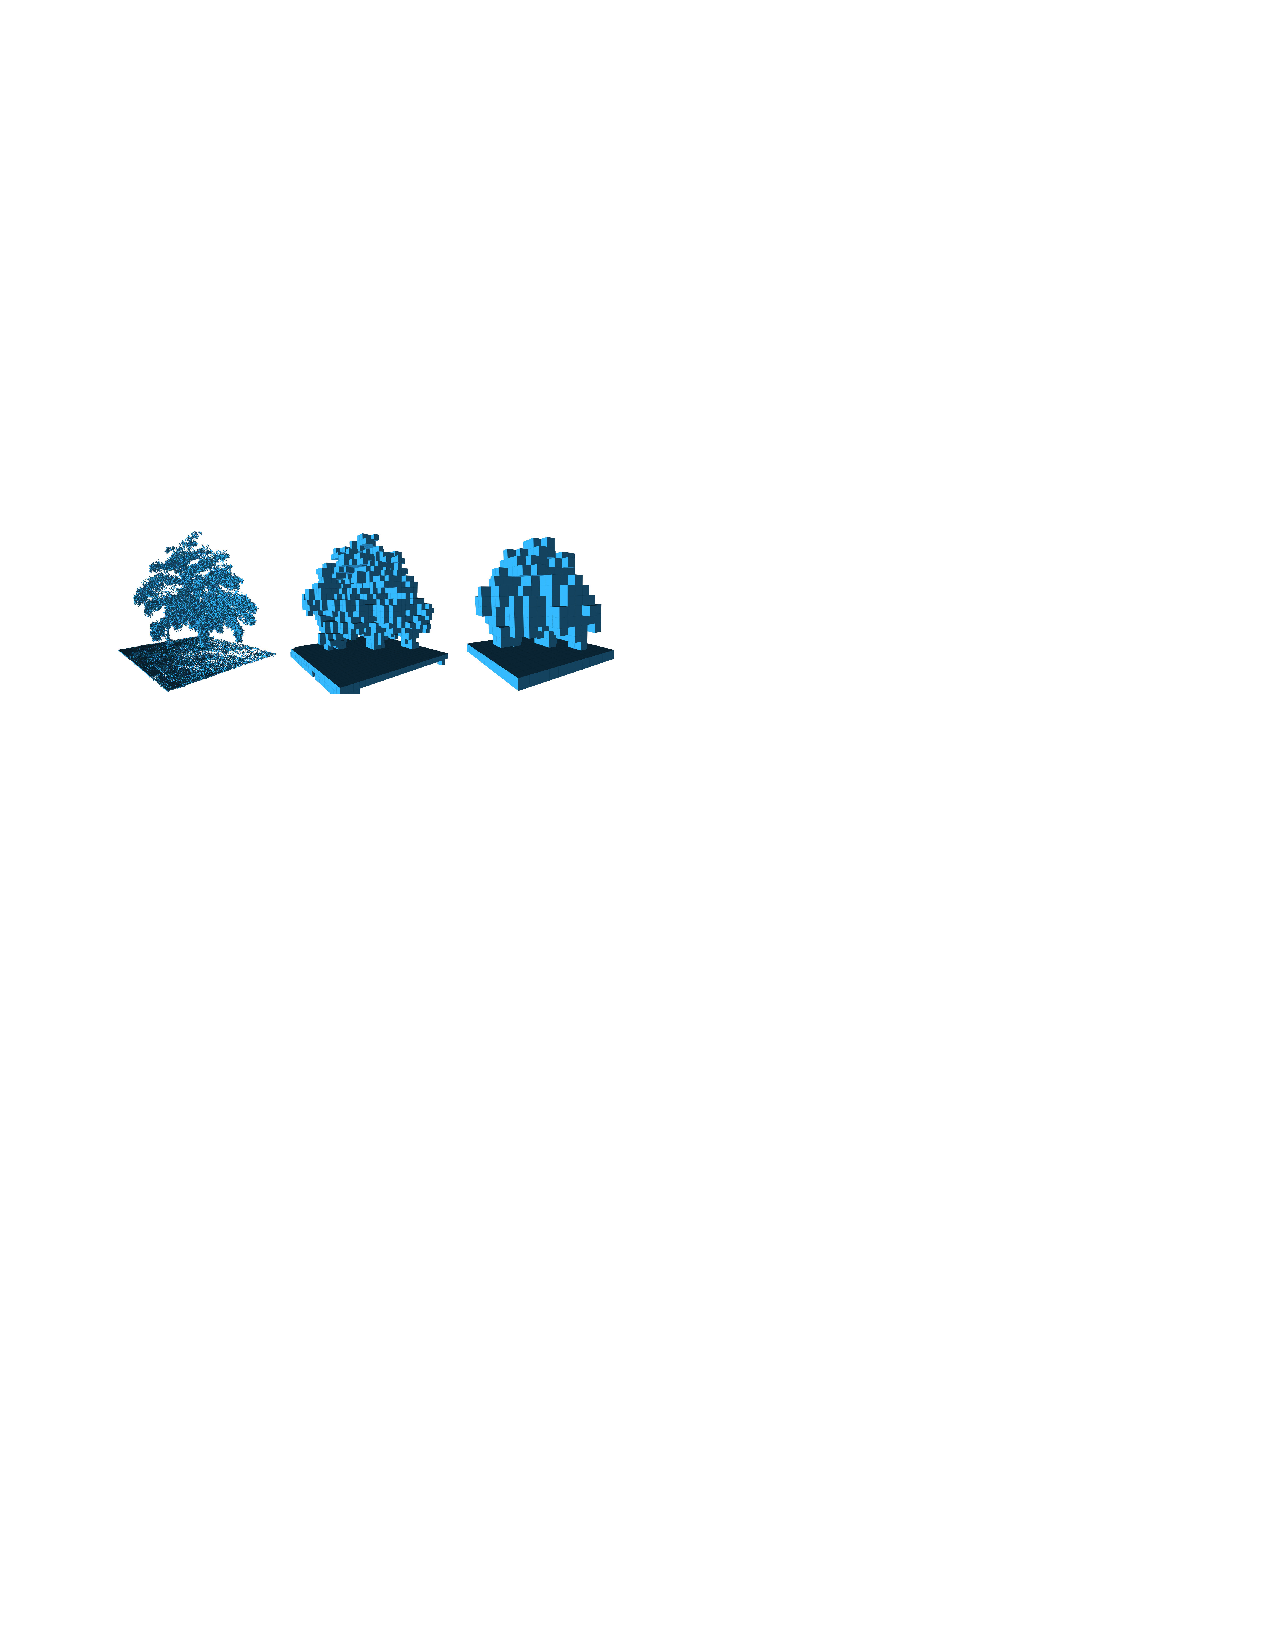
\includegraphics[width=3.5in,keepaspectratio]{treedepth.pdf}
    \caption{The resolution can be reduced by limiting the query 
             depth\cite{octomap}}
    \label{fig:treedepth}
  \end{figure}
  
  The algorithm for selecting the depth is proposed in Algorithm
  \ref{alg:bandwidth} and simply continues to degrade the resolution until
  there is enough bandwidth to transmit or until there resolution cannot be
  degraded further.
  
  \begin{algorithm}
  \caption{Algorithm for Determining Difference Depth}
  \label{alg:treedepth}
  \begin{algorithmic}
    \STATE \COMMENT {$O_0$ is the first octree}
    \STATE \COMMENT {$O_1$ is the second octree}
    \STATE \COMMENT {$d$ is the differences}
    \STATE \COMMENT {$B_d$ is the bandwidth required for the differences}
    \STATE \COMMENT {$B_a$ is the available bandwidth}
    \STATE \COMMENT {$T_u$ is the update period}
    \STATE $i\gets 0$
    \REPEAT
      \STATE $O_0 \prime = depth(O_0,height(O_0)-i)$
      \STATE $O_1 \prime = depth(O_1,height(O_1)-i)$
      \STATE $d = O_0 \prime \bigcup O_1 \prime $
      \STATE $B_d = size(d) * T_u$
      \STATE $B_a = currentAvailableBandwidth()$
      \STATE $i = i + 1$
    \UNTIL {$B_d\le B_a \| i = height(O_0) \| i = height(O_1)$}
    \RETURN $d$
  \end{algorithmic}
  \end{algorithm}
  
  The depth function simply returns a subtree of the given tree at the height given, and the height function gives the height of the tree specified.  The current available bandwidth function could be implemented in several ways, but the topic of available bandwidth estimation has been covered in the literature.\cite{prasad2003bandwidth}  The principal behind the bandwidth estimation is looking at metrics like round-trip-time, average delay, and throughput to determine the bandwidth currently available.
  
  \subsubsection{Octree Set Union}
  The final stage of synchronizing the server and client octrees is to unite
  the differences with the client octree. This is just a simple union
  operation and can be performed by simply inserting every voxel in the
  differences into the client map using the normal octree insertion
  method.\cite{meagher1982geometric}.
  
  \section{Results}
  In this section the paper describes the results of the three dimensional mapping and the experimental setups that were used.  Data was collected from multiple real platforms as well as simulated data.
  
  \subsection{Experimental Setup}
  \label{sec:experimental_setup}
  adsf
  
  \subsection{Simulated Environment}
  asdf
  
  \section{Future Work}
  Future work.
  
  \section{Conclusion}
  Conclusions
  
  \newpage
  
  \bibliographystyle{IEEEtran}
  \bibliography{citations}
  
  \begin{IEEEbiography}
    [{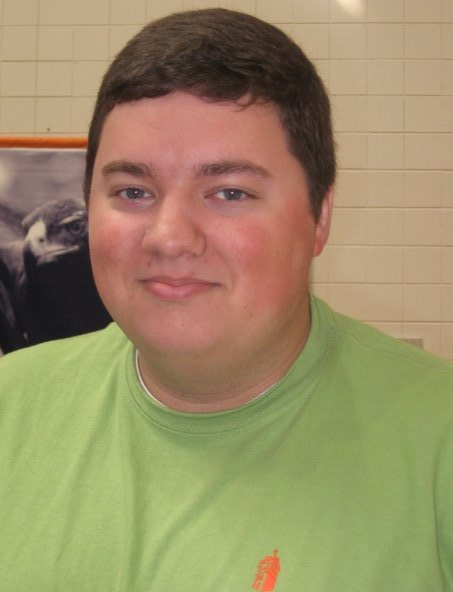
\includegraphics[height=1.25in,clip,keepaspectratio]{william.jpg}}]
    {William J. Woodall IV}
      William is a graduate research assistant at Auburn University and is
      pursuing his Master of Science in Software Engineering. He works for Dr.
      David Bevly of the Mechanical Engineering Department on Mobile Robotics
      and Advanced Teleoperation. William's research interests include mobile
      robotics, navigation and control, and perception.
  \url{http://williamjwoodall.com}
  \end{IEEEbiography}
  
\end{document}
